\section{Referencia de la Clase Pedido\-Cliente}
\label{classPedidoCliente}\index{PedidoCliente@{PedidoCliente}}
Almacena la informaci\'{o}n de un pedido de cliente.  


{\tt \#include $<$pedidocliente.h$>$}

Diagrama de herencias de Pedido\-Cliente\begin{figure}[H]
\begin{center}
\leavevmode
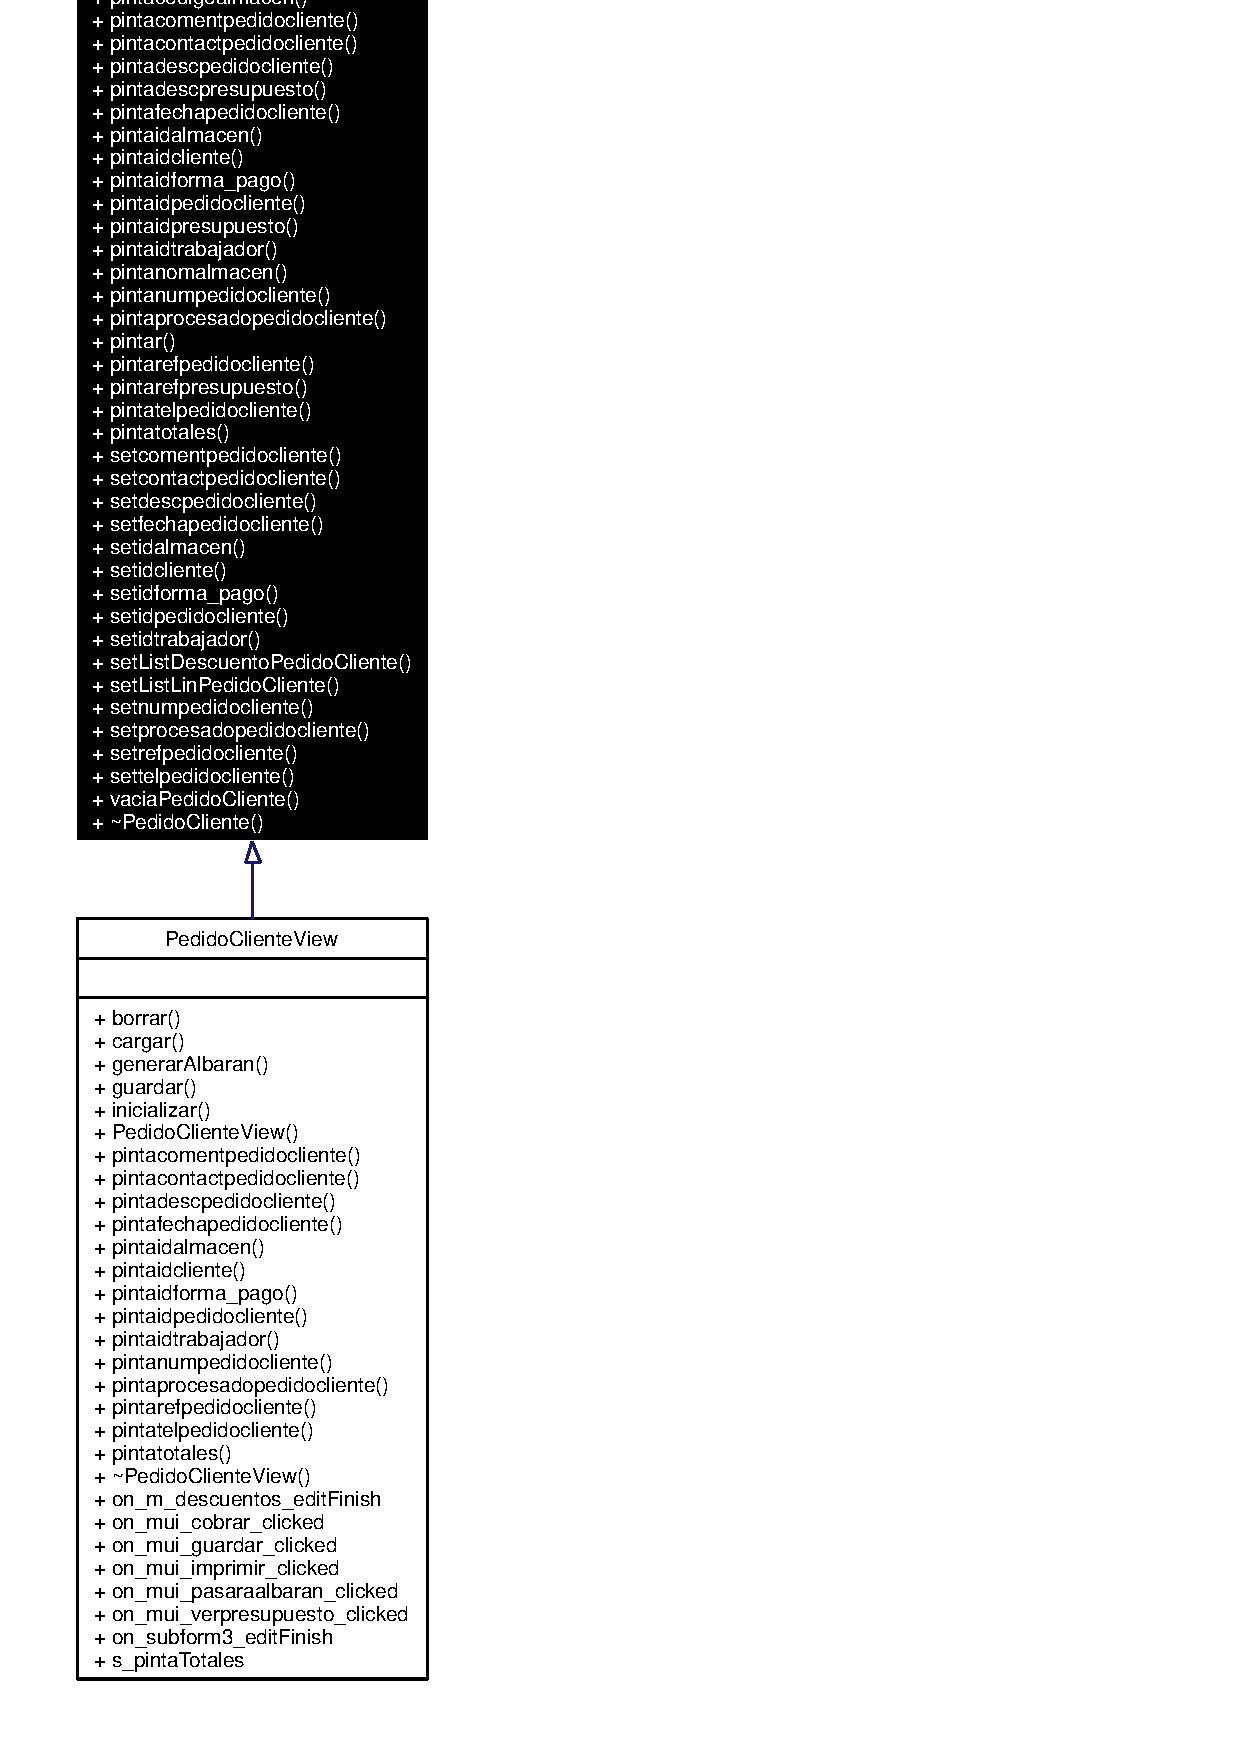
\includegraphics[width=103pt]{classPedidoCliente__inherit__graph}
\end{center}
\end{figure}
Diagrama de colaboraci\'{o}n para Pedido\-Cliente:\begin{figure}[H]
\begin{center}
\leavevmode
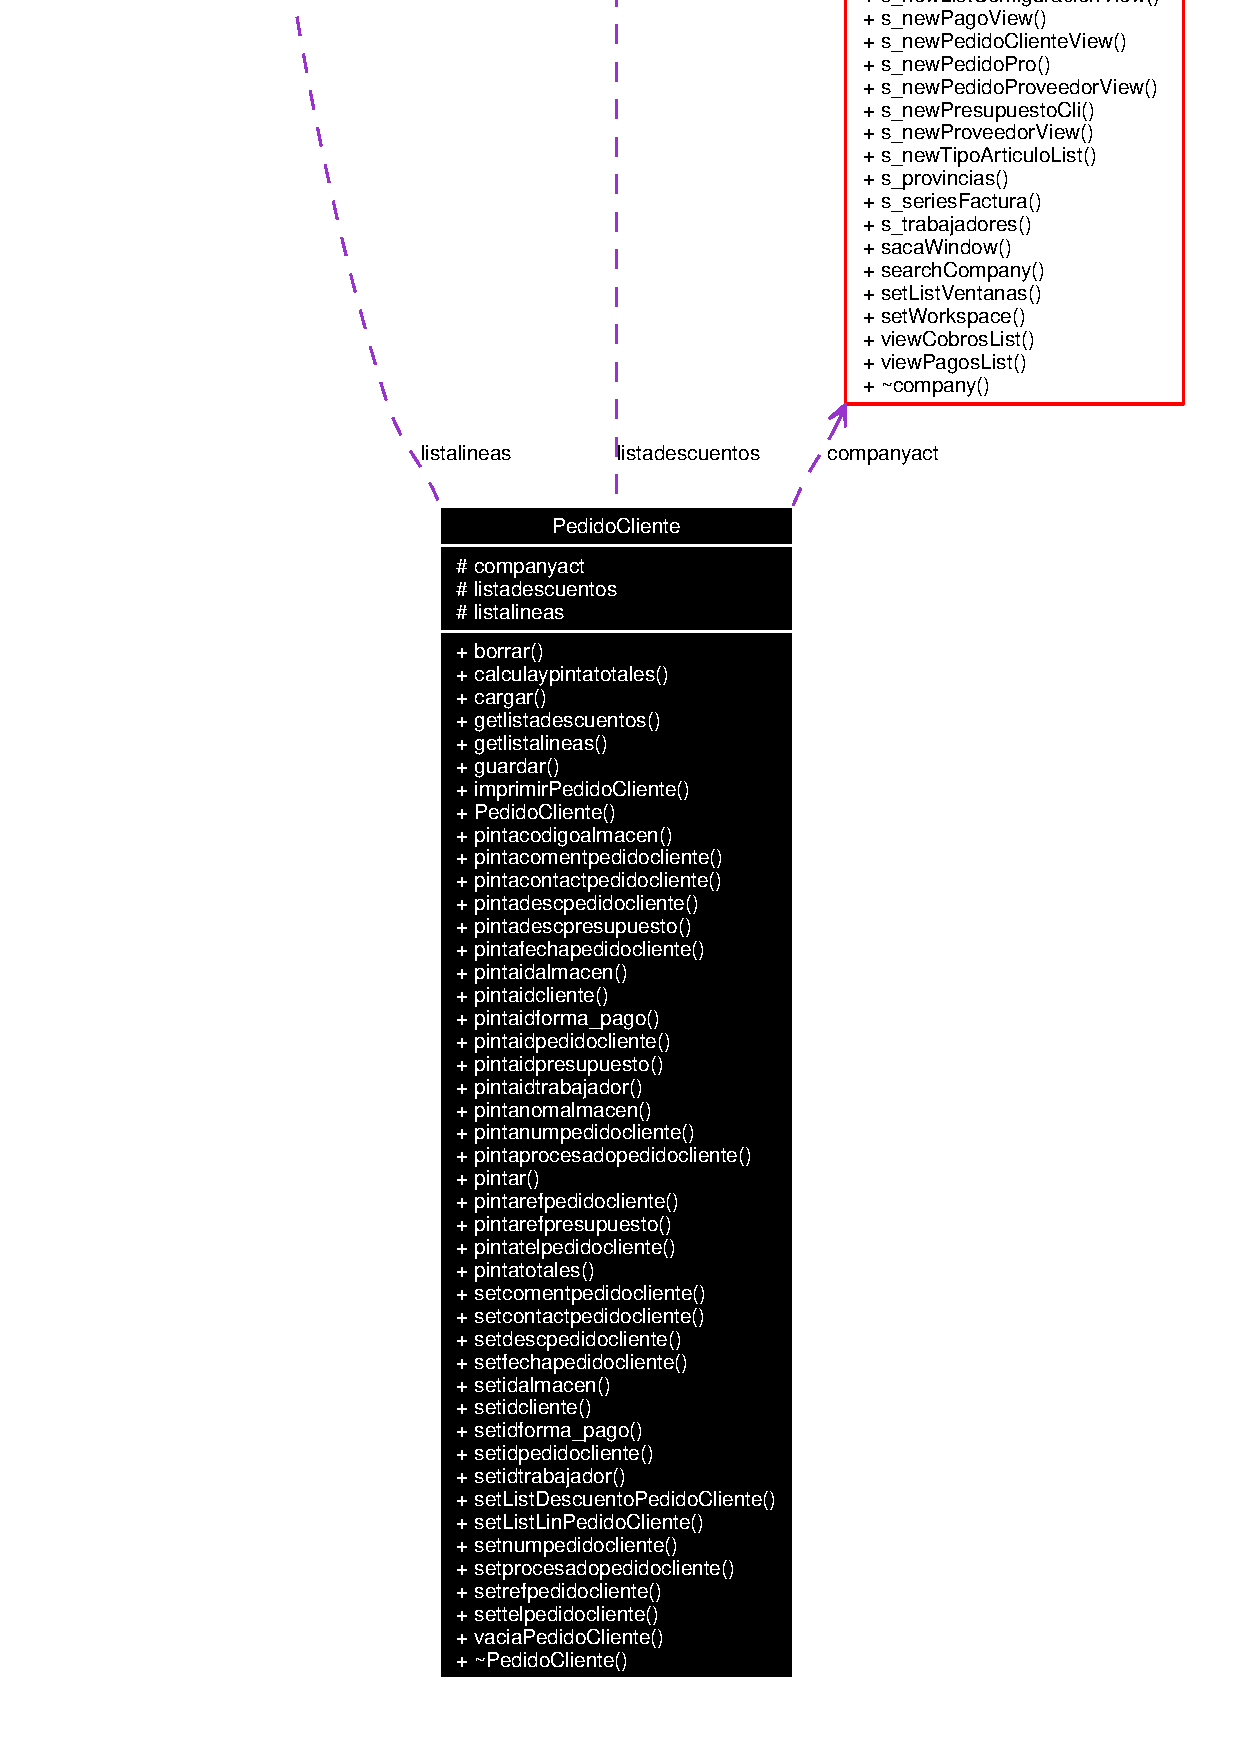
\includegraphics[width=284pt]{classPedidoCliente__coll__graph}
\end{center}
\end{figure}
\subsection*{M\'{e}todos p\'{u}blicos}
\begin{CompactItemize}
\item 
virtual int {\bf borrar} ()\label{classPedidoCliente_a0}

\item 
virtual void {\bf calculaypintatotales} ()
\item 
virtual int {\bf cargar} (QString)\label{classPedidoCliente_a2}

\begin{CompactList}\small\item\em Esta funcion carga un Pedido\-Cliente. \item\end{CompactList}\item 
{\bf List\-Descuento\-Pedido\-Cliente\-View} $\ast$ {\bf getlistadescuentos} ()\label{classPedidoCliente_a3}

\item 
{\bf List\-Lin\-Pedido\-Cliente\-View} $\ast$ {\bf getlistalineas} ()\label{classPedidoCliente_a4}

\item 
virtual int {\bf guardar} ()\label{classPedidoCliente_a5}

\item 
virtual void {\bf imprimir\-Pedido\-Cliente} ()
\item 
{\bf Pedido\-Cliente} ({\bf company} $\ast$)\label{classPedidoCliente_a7}

\item 
virtual void {\bf pintacodigoalmacen} (QString)\label{classPedidoCliente_a8}

\item 
virtual void {\bf pintacomentpedidocliente} (QString)\label{classPedidoCliente_a9}

\item 
virtual void {\bf pintacontactpedidocliente} (QString)\label{classPedidoCliente_a10}

\item 
virtual void {\bf pintadescpedidocliente} (QString)\label{classPedidoCliente_a11}

\item 
virtual void {\bf pintadescpresupuesto} (QString)\label{classPedidoCliente_a12}

\item 
virtual void {\bf pintafechapedidocliente} (QString)\label{classPedidoCliente_a13}

\item 
virtual void {\bf pintaidalmacen} (QString)\label{classPedidoCliente_a14}

\item 
virtual void {\bf pintaidcliente} (QString)\label{classPedidoCliente_a15}

\item 
virtual void {\bf pintaidforma\_\-pago} (QString)\label{classPedidoCliente_a16}

\item 
virtual void {\bf pintaidpedidocliente} (QString)\label{classPedidoCliente_a17}

\item 
virtual void {\bf pintaidpresupuesto} (QString)\label{classPedidoCliente_a18}

\item 
virtual void {\bf pintaidtrabajador} (QString)\label{classPedidoCliente_a19}

\item 
virtual void {\bf pintanomalmacen} (QString)\label{classPedidoCliente_a20}

\item 
virtual void {\bf pintanumpedidocliente} (QString)\label{classPedidoCliente_a21}

\item 
virtual void {\bf pintaprocesadopedidocliente} (QString)\label{classPedidoCliente_a22}

\item 
virtual void {\bf pintar} ()\label{classPedidoCliente_a23}

\item 
virtual void {\bf pintarefpedidocliente} (QString)\label{classPedidoCliente_a24}

\item 
virtual void {\bf pintarefpresupuesto} (QString)\label{classPedidoCliente_a25}

\item 
virtual void {\bf pintatelpedidocliente} (QString)\label{classPedidoCliente_a26}

\item 
virtual void {\bf pintatotales} (Fixed, Fixed, Fixed, Fixed)\label{classPedidoCliente_a27}

\item 
void {\bf setcomentpedidocliente} (QString val)\label{classPedidoCliente_a28}

\item 
void {\bf setcontactpedidocliente} (QString val)\label{classPedidoCliente_a29}

\item 
void {\bf setdescpedidocliente} (QString val)\label{classPedidoCliente_a30}

\item 
void {\bf setfechapedidocliente} (QString val)\label{classPedidoCliente_a31}

\item 
void {\bf setidalmacen} (QString val)\label{classPedidoCliente_a32}

\item 
void {\bf setidcliente} (QString val)\label{classPedidoCliente_a33}

\item 
void {\bf setidforma\_\-pago} (QString val)\label{classPedidoCliente_a34}

\item 
void {\bf setidpedidocliente} (QString val)\label{classPedidoCliente_a35}

\item 
void {\bf setidtrabajador} (QString val)\label{classPedidoCliente_a36}

\item 
void {\bf set\-List\-Descuento\-Pedido\-Cliente} ({\bf List\-Descuento\-Pedido\-Cliente\-View} $\ast$a)\label{classPedidoCliente_a37}

\item 
void {\bf set\-List\-Lin\-Pedido\-Cliente} ({\bf List\-Lin\-Pedido\-Cliente\-View} $\ast$a)\label{classPedidoCliente_a38}

\item 
void {\bf setnumpedidocliente} (QString val)\label{classPedidoCliente_a39}

\item 
void {\bf setprocesadopedidocliente} (QString val)\label{classPedidoCliente_a40}

\item 
void {\bf setrefpedidocliente} (QString val)\label{classPedidoCliente_a41}

\item 
void {\bf settelpedidocliente} (QString val)\label{classPedidoCliente_a42}

\item 
void {\bf vacia\-Pedido\-Cliente} ()\label{classPedidoCliente_a43}

\end{CompactItemize}
\subsection*{Atributos protegidos}
\begin{CompactItemize}
\item 
{\bf company} $\ast$ {\bf companyact}\label{classPedidoCliente_p0}

\item 
{\bf List\-Descuento\-Pedido\-Cliente\-View} $\ast$ {\bf listadescuentos}\label{classPedidoCliente_p1}

\item 
{\bf List\-Lin\-Pedido\-Cliente\-View} $\ast$ {\bf listalineas}\label{classPedidoCliente_p2}

\end{CompactItemize}


\subsection{Descripci\'{o}n detallada}
Almacena la informaci\'{o}n de un pedido de cliente. 



\subsection{Documentaci\'{o}n de las funciones miembro}
\index{PedidoCliente@{Pedido\-Cliente}!calculaypintatotales@{calculaypintatotales}}
\index{calculaypintatotales@{calculaypintatotales}!PedidoCliente@{Pedido\-Cliente}}
\subsubsection{\setlength{\rightskip}{0pt plus 5cm}void Pedido\-Cliente::calculaypintatotales ()\hspace{0.3cm}{\tt  [virtual]}}\label{classPedidoCliente_a1}


Impresion de los contenidos.

Impresion de los descuentos. \index{PedidoCliente@{Pedido\-Cliente}!imprimirPedidoCliente@{imprimirPedidoCliente}}
\index{imprimirPedidoCliente@{imprimirPedidoCliente}!PedidoCliente@{Pedido\-Cliente}}
\subsubsection{\setlength{\rightskip}{0pt plus 5cm}void Pedido\-Cliente::imprimir\-Pedido\-Cliente ()\hspace{0.3cm}{\tt  [virtual]}}\label{classPedidoCliente_a6}


Copiamos el archivo.

Copiamos el logo.

Linea de totales del presupuesto.

Impresion de la tabla de contenidos.

Impresion de los descuentos.

Impresion de los totales.

Rellena el primer tr de titulares.

Rellena el segundo tr de cantidades. 

La documentaci\'{o}n para esta clase fu\'{e} generada a partir de los siguientes archivos:\begin{CompactItemize}
\item 
pedidocliente.h\item 
pedidocliente.cpp\end{CompactItemize}
